
\section{Results}

In order to get a representation of the mechanism we run 300 randomly initiated scenarios. The experiemental setup is one such that it is possible to add more datapoints at a later date. From each simulation the no diagonal elements of the jacobian are used to construct a graph representative of the aggregated hourly means of the simulation output. Each of these graphs is then run through the infomap algorithm and a grouping/clustering produced. To select the best possible grouping, each infomap is run 100 times, where the result with the best fit (shortest codelength) is taken - this is an optional parameter on the algorithm.

\subsection{The co-grouping network}

To aggregate the groupings produced by each algorithm an $n\times n$ matrix is created for each of the $n$ species in the mechanism. This is treated as a graph relational matrix, whereupon if species A is in the same group as species B, then a link (or value +1) is added to the [A,B] (A\ce{->}B) and [B,A] (B\ce{->}A) column. Using this matrix format it is possible to then generate a graph showing the relationship between species that were clustered in the same group.

Using this matrix it is then possible to create a network, \autoref{fig:infomapprune}a, which can progressively be filtered to represent only the nodes which are consistently paired together. Using prior knowledge that changes in chemistry follow a daytime and nightime regeme, we select only relationships that appear in over 45\% of all the infomap runs.

\begin{figure}[H]
\begin{subfigure}[t]{.5\textwidth}
  \centering
  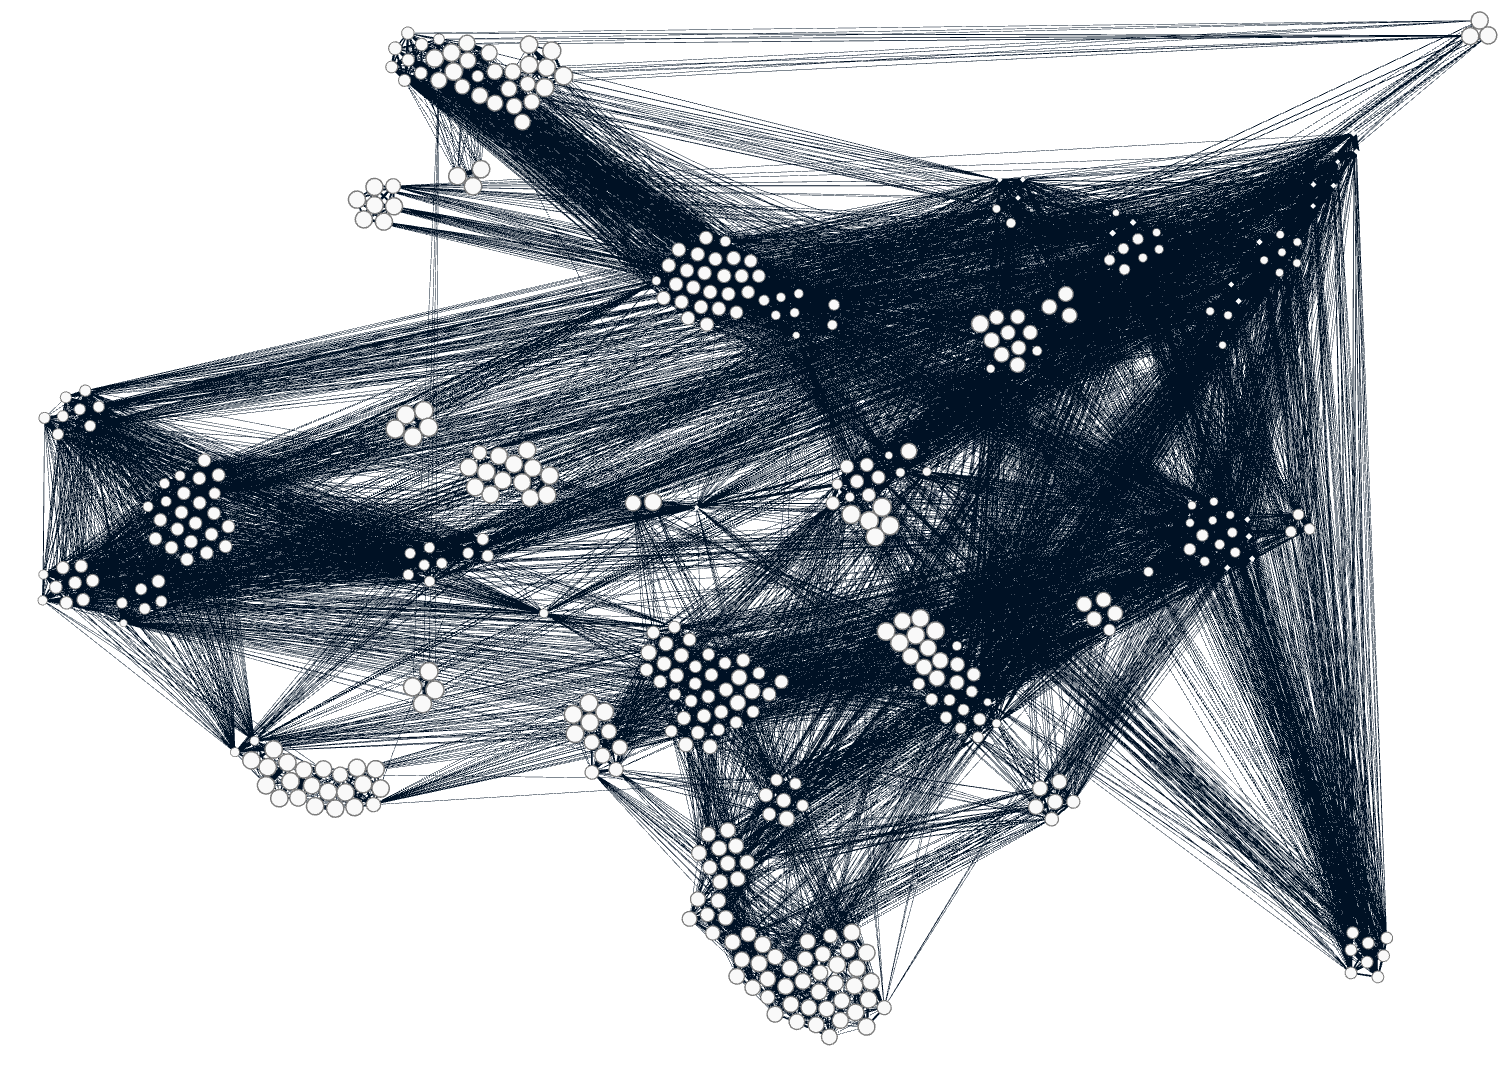
\includegraphics[width=\textwidth]{fig/c1.png}
  \caption{Full Graph}
\end{subfigure}%
\begin{subfigure}[t]{.5\textwidth}
  \centering
  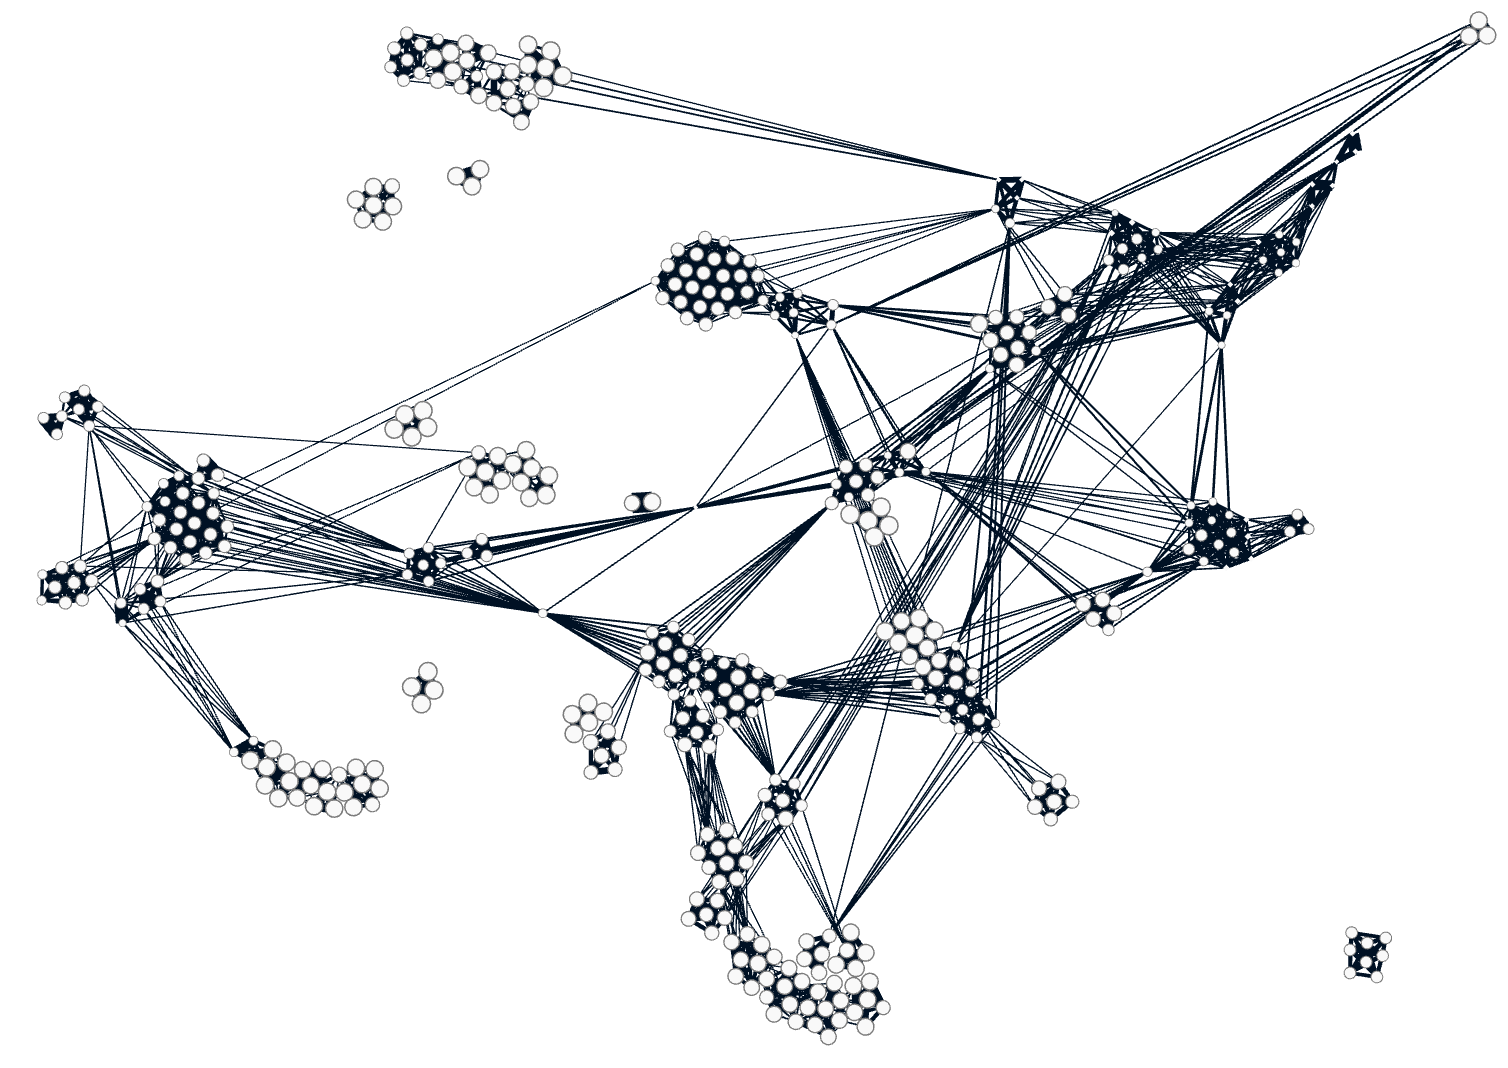
\includegraphics[width=\textwidth]{fig/c2.png}
  \caption{>10\% of graphs}
\end{subfigure}%\\

\begin{subfigure}[t]{.5\textwidth}
  \centering
  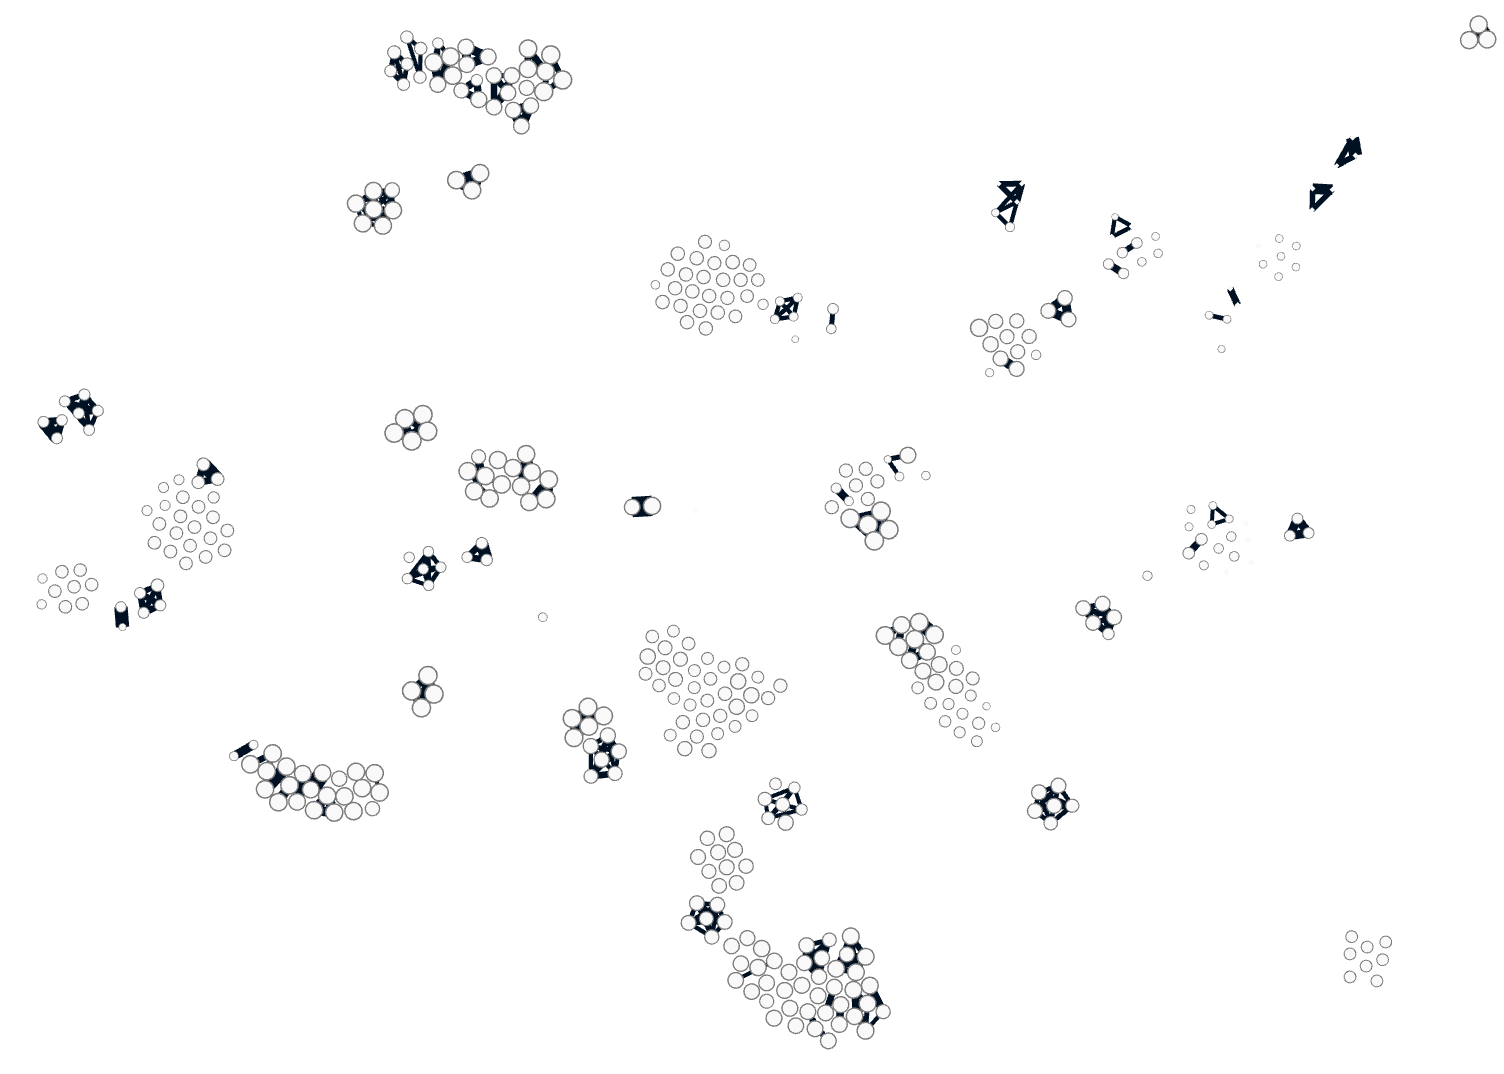
\includegraphics[width=\textwidth]{fig/c3.png}
  \caption{>20\%of graphs}
\end{subfigure}%
\caption{\textbf{Filetering the infomap clustering relationship matrix/graph} How the clutering relationship network changes as weak links (links between species which do not appear in many of the infomap groupings) are removed. }
\label{fig:infomapprune}
\end{figure}

\subsection{Comparing daytime and nightime groups}
Having determined a set of species which are continuously clustered for over 45\% of our simulation results, it is next important to see how these compare against those as part of a dirunal split. To this the output of the infomap clusters for midday and midnight are extracted. We then make use of an alluvial diagram. This is a cross between a parallel line plot and a sanky diagram and is often used to show changes in categorical data. This makes them particularly suitable for showing the changes of clusters within a temporal networks, as has been shown in \citep{alluvial}.

\autoref{fig:alluvial} shows the




\begin{figure}[H]
    \centering
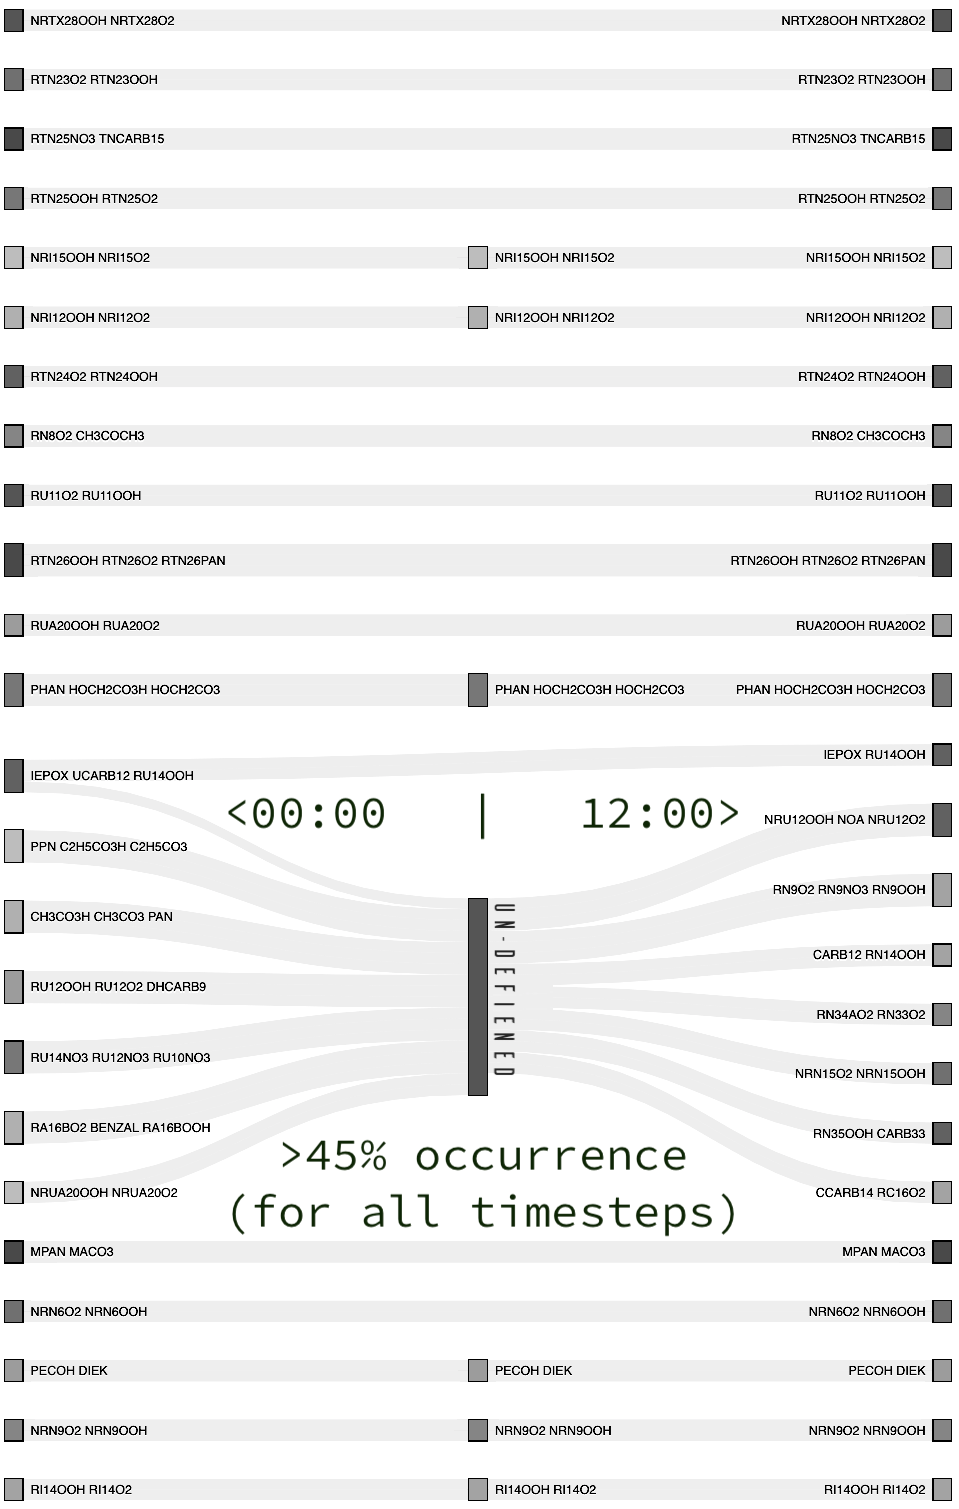
\includegraphics[width=.9\textwidth]{fig/alluvial.png}
\caption{\textbf{An alluvial diagram showing the changes in clusters between noon and midnight.} On the left are all groups that apear in >45\% of the midnight simulation results. On the right are groups which appear >45\% of the midday results. In the middle exist the clusters extracted which appear in >45\% of all runs. Here it is seen that there exist a series of species which may exist in daytime or nighttime chemistry, but do not persist between both. }
\label{fig:alluvial}
\end{figure}



\subsection{Determining cluster suitabiltiy}
Having selected clusters that appear for most graphs in the network, it is now important to assess the suitability of each node for being lumped together. 



Similarly the lifetimes of each species are extracted from the diagonal of the jacobian matrix. Using these the euclidian and cosine similarities are calculated and can be used to determine how well suited a species pair is for beign lumped together.
